\chapter{Implementation}\label{chap:implementation}
In the following a brief introduction is given to the important data structures
and algorithms that are used in the MRChem program. This will introduce the 
nomenclature used in the rest of the thesis. The code is written in C++, utilizing the 
consepts of object-orientation and generic programming, where for instance the 
dimension appears as a template parameter, which means that the code is immediately 
applicable to any dimension, although some algorithms are specialized and optimized 
for $d=3$.

Due to the inherent high demands on memory and computational resources that comes
with all real-space numerical methods, the code relies heavily on 
parallel algorithms and data distribution. In the current code data distribution is
handled by the Message-Passing Interface (MPI) protocol, and further work load
distribution is provided by an additional shared memory (OpenMP) parallelization 
on top. The parallel implementation and the performance of the code is discussed 
fully in publication 1.

\section{Data structures}
\subsection{\Node}
The \node is the multidimensional box on which the set of
scaling and wavelet functions that share the same support are defined. The 
\node is specified by its scale $n$, which gives its size 
($[0,2^{-n}]^d$) and translation vector $\bs{l} = (l_1,l_2,\dots,l_d)$, 
which gives its position. The \node holds the $(k+1)^d$ scaling 
coefficients and $(2^d-1)(k+1)^d$ wavelet coefficients that share the same 
scale and translation. It will also keep track of its parent and all $2^d$ 
children \nodes, giving the \nodes a tree-like structure. 

\subsection{\Tree}
The \tree data structure is a collection of \nodes that makes up a function.
In order to minimize the memory requirements, all variables that are common to
all \nodes (like polynomial order, number of coefficients, type of scaling 
functions, etc) are stored in the \tree structure. The \tree keeps the entire 
set of \nodes, from root to leaf, and each \node keeps both the scaling and 
wavelet coefficients. This means that there is a redundancy in the function 
representation as the multiresolution representation in Eq.~(\ref{eq:multires})
requires scaling coefficients only at the coarsest scale. However, it proves 
more efficient to keep all scaling coefficients in memory rather than obtaining
them by the filter operations of Eq.~(\ref{eq:twoscalerelations}), as they are 
needed e.g. in the non-standard operator application.

\subsection{Parallel data distribution}
As the data storage requirements of real-space methods quickly exceeds the 
available memory on a single computational device, it eventually becomes 
necessary to distribute the data that is contained in the full \tree 
representation of a function among the memory of several computers (hosts). 
In the multiwavelet basis the function representations are conveniently 
partitioned into equally sized portions (equal in terms of memory, not 
spatial extension), and data distribution is achieved by dividing these
\nodes among the available hosts.

There are several possible strategies for how the \nodes could be distributed
and we have chosen one that leads to strictly connected domains, in the sense 
that all \nodes belonging to a given host is connected (share a common vertice,
not necessarily on the same scale) to at least one other \node owned by the same 
host. This ensures that the real-space domain of a given host will be localized 
in space, with the motivation that the interaction between hosts could be limited
to involve only near neighbors, and thus hopefully reduce the need for communication
between hosts.

In order to achieve this localization we traverse the \tree following a space-filling
path, assigning \nodes to hosts as we go. By following a so-called Hilbert 
path~\cite{Griebel}, we obtain a continuous curve with good locality properties, that
can be partitioned among the hosts. The construction of the curve is done recursively,
going through the $2^d$ children of each \node in a specific order. Using bit notation
(one bit for each dimension), the natural ordering (Lebesgue) will lead to a 
discontinuous path. For $d=2$ this is shown as the Z shape of the bit sequence 
(00, 01, 10, 11) in figure \ref{fig:lebesgue}. A corresponding (there are several 
possebilities) Hilbert path through the four children in two dimensions could be the 
bit sequence (00, 10, 11, 01) shown in the first panel in figure \ref{fig:hilbert}. 
In order to keep the continuouity as the path is recursively refined, the order in 
which the children are traversed needs to be adapted, and will depend on the position 
of the parent among its siblings, as shown in figure \ref{fig:hilbert}.

\begin{figure}
    \centering
    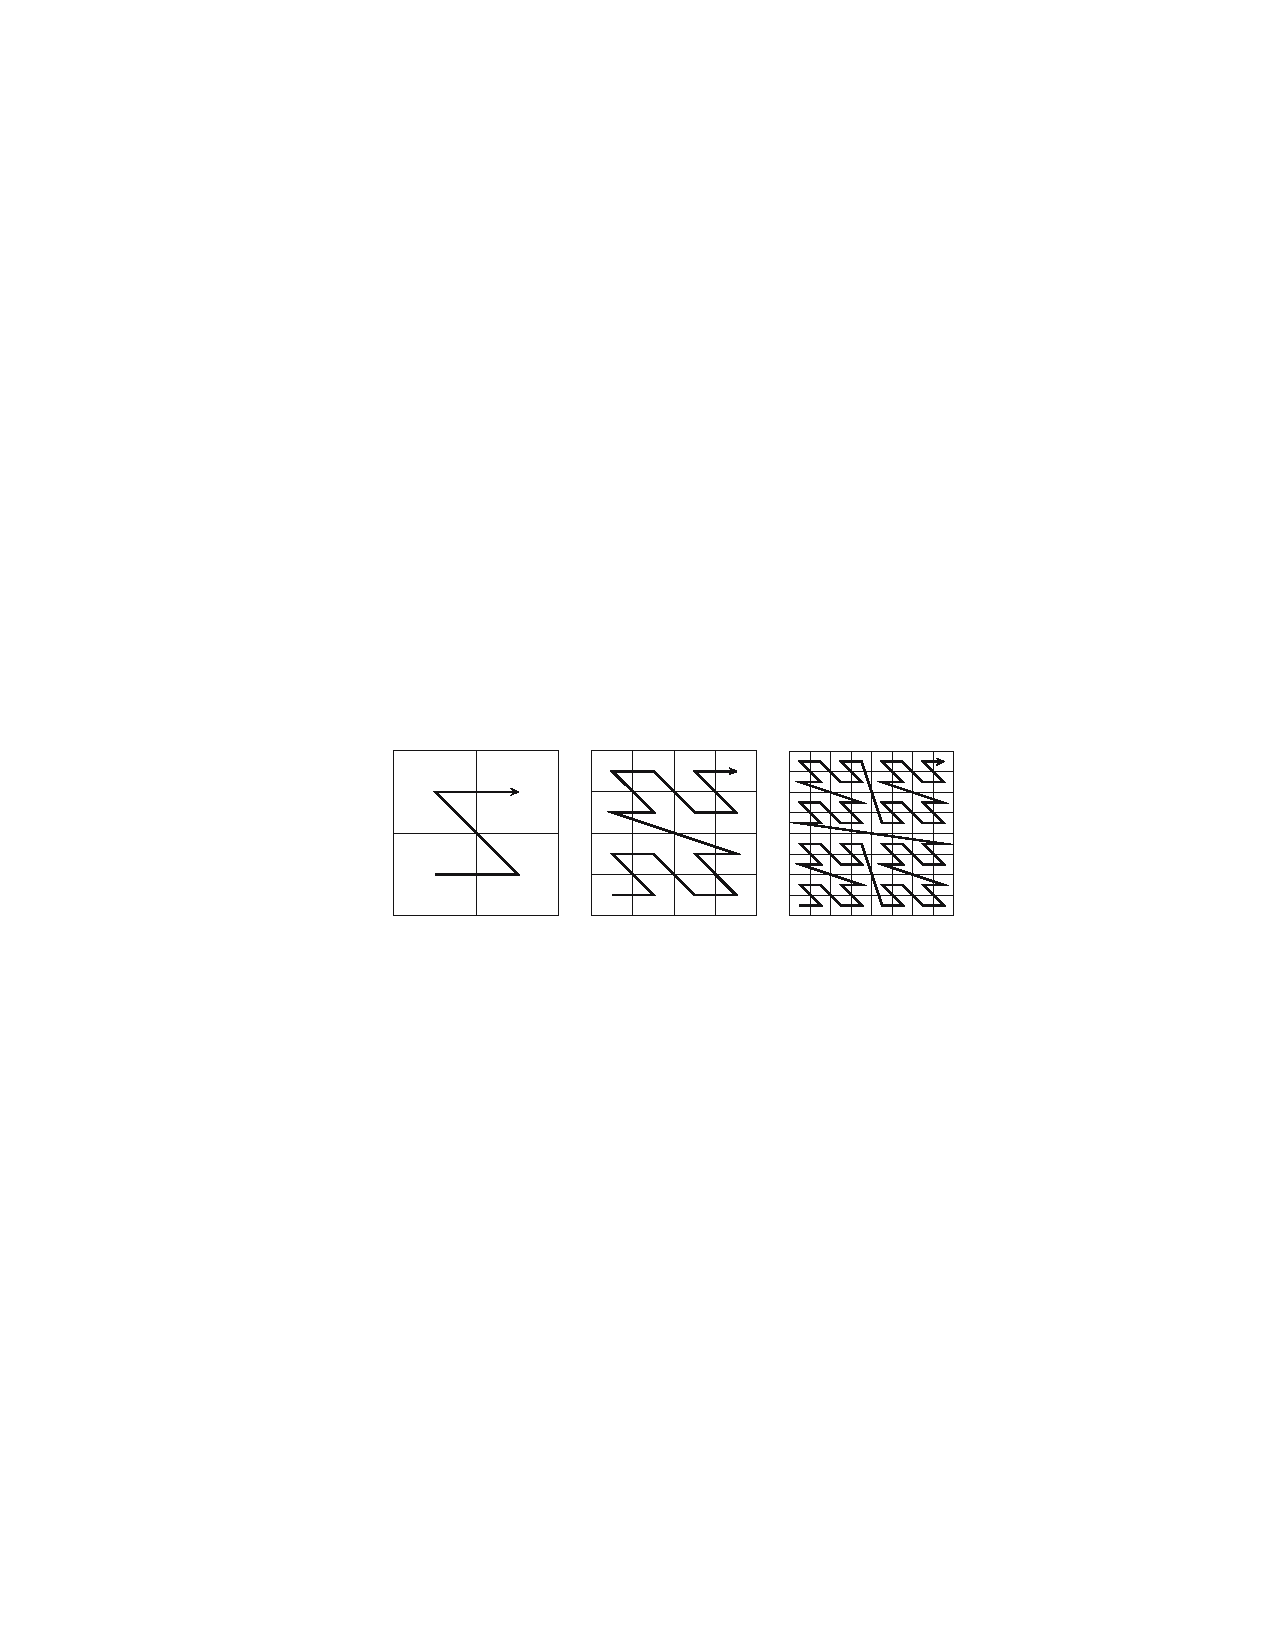
\includegraphics[scale=1.0, viewport = 150 350 500 435, clip]{figures/lebesgue.pdf}
    \caption{\footnotesize{Three refinement levels in the construction of the Lebesgue 
	curve in 2D.}}
    \label{fig:lebesgue}
\end{figure}
\begin{figure}
    \centering
    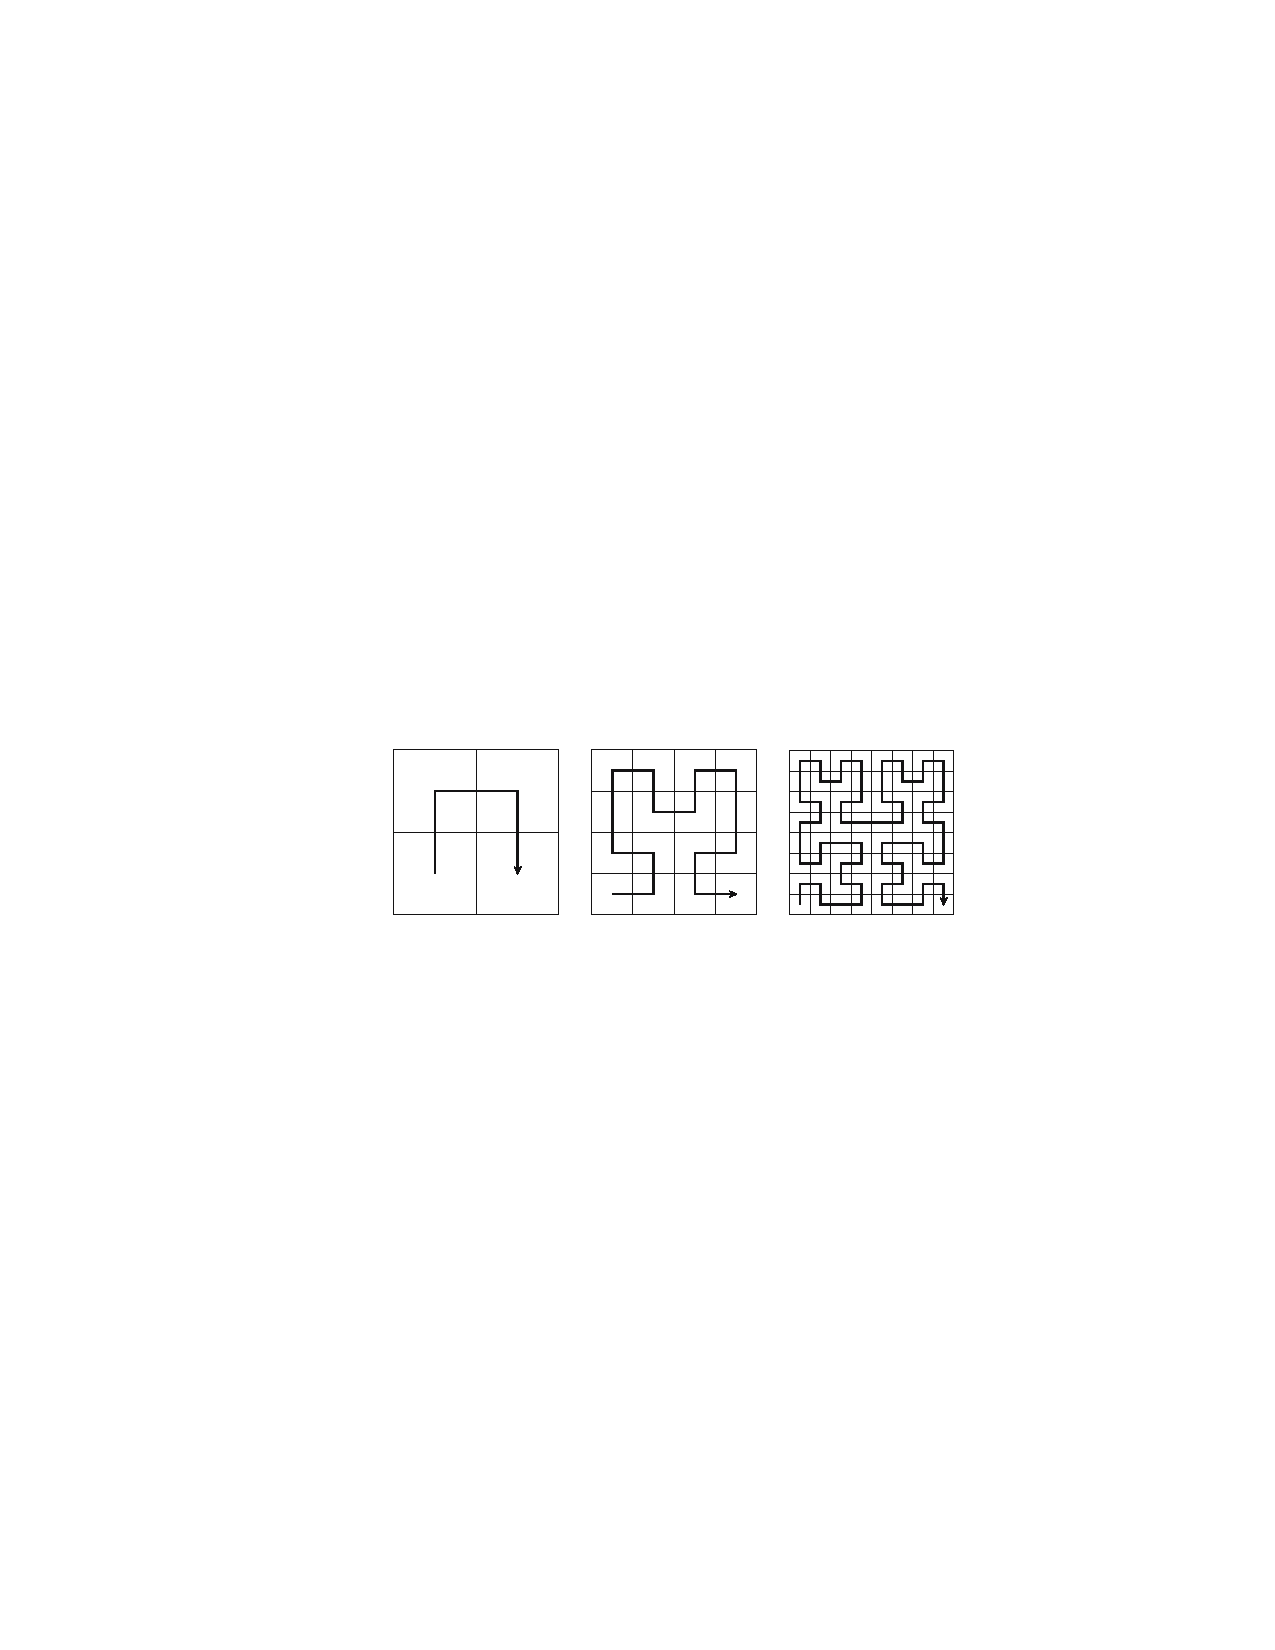
\includegraphics[scale=1.0, viewport = 150 350 500 435, clip]{figures/hilbert.pdf}
    \caption{\footnotesize{Three refinement levels in the construction of the Hilbert 
	curve in 2D.}}
    \label{fig:hilbert}
\end{figure}

\section{Adaptive algorithm}
\begin{algorithm}
    \footnotesize
    \caption{Generation of adaptive multiwavelet representation of a function}
    \label{alg:function}
    \begin{algorithmic}[1]
	\STATE create \tree skeleton of empty \nodes
	\STATE MPI: distribute leaf \nodes among hosts through Hilbert path
	\STATE MPI: create list of local \nodes owned by \emph{this} host
	\WHILE{number of local \nodes on current iteration $N_i>0$}
	    \STATE OpenMP: divide local \nodes among available processors
	    \FOR{each \node at current iteration}
		\STATE compute scaling and wavelet coefficients
		\IF{\node needs to be refined}
		    \STATE mark \node as non-terminal
		    \STATE allocate children \nodes
		    \STATE update list of local \nodes for next iteration
		\ELSE
		    \STATE mark \node as terminal
		\ENDIF
	    \ENDFOR
	    \STATE increment iteration
	\ENDWHILE
    \end{algorithmic}
\end{algorithm}

\noindent
Algorithm \ref{alg:function} used to obtain adaptive representations of functions 
was originally presented in \cite{Frediani}, but is here extended to include 
parallelization. The first lines in this algorithm are very important in order to 
ensure a good
load balancing among MPI hosts. By utilizing some a priori knowledge of the
function that is about to be buildt, we try to estimate the final tree structure
as closely as possible before calculating any coefficients. In this way we have
a lot more flexibility when it comes to parallel distribution of data and work load 
in all iterations. Without this preprocessing step, the first three iterations would 
contain one, eight and 64 \texttt{nodes}, respectively, allowing little freedom in
parallel computations. It is important in this step to capture the global structure
of the function (where in space is high level of refinement needed), as this initial
tree skeleton is used in the data distribution among MPI hosts and all subsequent
additional refinent is done locally on each host (although some load balancing can
be preformed by redistribution of data if needed). How to construct this skeleton
depends on the function, and will be discussed in the following sections.

The algorithm consists of two loops, the first iteration will add levels of 
refinement on top of the initial skeleton wherever necessary in order to guarantee
the overall accuracy of the representation. This loop terminates when no further
refinement is needed. The second loop runs over the \nodes present at the current 
iteration (only local nodes that belong to the given MPI host), and these are 
distributed among the available processors (OpenMP) at the given host. Once the 
scaling/wavelet coefficients of a given \node are known, a split check is performed 
based on the desired precision. If the \node does not satisfy the accuracy criterion, 
it is marked as non-terminal and its children \nodes are allocated and added to the 
list of \nodes needed in the next iteration. If the \node does not need to be split, 
it is marked as terminal and no children \nodes are allocated. In this way, once the 
loop over \nodes on one iteration is terminated, the complete list of \nodes needed 
in the next iteration has been obtained. The \tree is grown until no \nodes are 
needed at the next iteration.

There are two points in the algorithm that need to be elaborated further, the first 
being the actual computation of the coefficients (line 7). This can be done in 
many ways, e.g. projection or by operator application, and will be treated in 
the subsequent sections. 

The second point is how to perform the split check (line 8), which is used to decide 
whether or not the function is represented accurately enough on the current 
\texttt{node}, based on a predefined relative precision $\epsilon$. Formally, this 
relative precision requires that 
\begin{equation}
    \|f-\scalingrep{f}{n}\| < \epsilon \|f\|
\end{equation}
However, this check cannot be performed since the \emph{true} function $f$ is 
generally not known. Instead we will use the norm of the wavelet projections as a
measure of the accuracy of the representation. Specifically, the norm of the wavelet 
coefficients on one \node is used as a measure for the accuracy of the part of the
function represented by this \texttt{node}, and we require that
\begin{equation}
    \|\bs{\waveletcoef}^n_{\bs{l}}\| < \frac{\epsilon}{2^{n/2}} \|\scalingrep{f}{n}\|
\end{equation}
The local, disjoint support of the wavelet basis ensures that the global error of
the representation can be controlled by locally truncating the wavelet expansion,
allowing a fully on-the-fly adaptive algorithm. This reduces the number of expansion 
coefficients needed to represent the function to the given accuracy dramatically 
compared to the uniform high-resolution representation in Eq.~(\ref{eq:highres}).
In practical calculations one can easily get significant contribution over a range
of ten length scales, and a uniform grid in three dimensions at scale $n=10$ would
require $(2^d)^n = 8^{10} \sim 10^9$ \nodes, while a typical multi-resolution
representation requires in the order of $10^2-10^4$ \nodes per scale.

The presented algorithm is very general, and is used to build adaptive 
representations of functions regardless of how the expansion coefficients are 
obtained, and later in the chapter we will look at different ways of doing this.

\section{Choice of basis functions}
Before we can describe how to calculate expansion coefficients we need to specify
the type of scaling and wavelet functions that is used in the multiresolution 
analysis. In principal, any polynomial basis that span the appropriate scaling
\scalingspace{n} and wavelet \waveletspace{n} spaces can be used, and in the original 
construction Alpert \cite{Alpert} used Legendre polynomials as scaling basis, but in 
a later work, Alpert \etal \cite{Alpert} introduced an alternative basis with 
interpolating properties. Both scaling bases have been implemented, but in practice
only the latter is used, because of its superior numerical efficiency. The choice of
wavelet basis follows that of Alpert\cite{Alpert}.

\subsection{Legendre scaling functions}
The Legendre polynomials $\lbrace L_j(x)\rbrace_{j\in \mathbb{N}}$ are a family of 
functions, defined on the interval $[-1,1]$. The functions are orthogonal with 
respect to the $L^2([-1,1])$ inner product
\begin{equation}
    \int_{-1}^{1} L_i(x)L_j(x) \ud x = 0, \qquad i \neq j
\end{equation}
but they are usually normalized such that $L_j(1) = 1$. The polynomials can be 
constructed by induction
\begin{align}
    L_0(x) &= 1\\
    L_1(x) &= x\\
    L_{j+1}(x) &= \frac{2j+1}{j+1}xL_j(x) - \frac{j}{j+1}L_{j-1}
\end{align}
and the \emph{Legendre scaling functions} $\scaling_j^L$ are obtained by dilation 
and translation to the unit interval, followed by $L^2$ normalization
\begin{equation}
    \scaling_j^L(x) = \sqrt{2j+1}L_j(2x-1),\qquad x \in [0,1]
\end{equation}
This is the original construction of scaling functions by Alpert\cite{Alpert}.

\subsection{Interpolating scaling functions}
Alpert \etal\cite{Alpert} presented an alternative set of scaling functions 
with interpolating properties. These \emph{Interpolating scaling functions} 
$\scaling_j^I$ are based on the Legendre scaling functions $\lbrace \scaling_j^L
\rbrace_{j=0}^k$, and the roots $\lbrace x_j\rbrace_{j=0}^k$ and weights
$\lbrace \omega_j \rbrace_{j=0}^k$ of the Gauss-Legendre quadrature of order 
$k+1$, and are constructed as the linear combinations
\begin{equation}
    \label{eq:interpolating}
    \scaling_j^I(x) = \sqrt{\omega_j}\sum_{i=0}^{k} 
	\scaling_i^L(x_j)\scaling_i^L(x),\qquad x \in [0,1]
\end{equation}
This construction leads to orthogonality on the unit interval, as well as the 
interpolating property
\begin{equation}
    \label{eq:interprop}
    \scaling_j^I(x_i) = \frac{\delta_{j,i}}{\sqrt{\omega_i}}
\end{equation}
which will prove important for numerical efficiency. A detailed discussion on 
the properties of Interpolating wavelets can be found in Donoho \cite{Donoho}.

\subsection{Wavelet basis}
There are two necessary constraints in the construction of the wavelet functions
$\wavelet_j$: they must be orthogonal to the scaling functions and orthogonal among 
themselves. It turns out that this is not sufficient to determine the wavelet functions
uniquely, so Alpert~\cite{Alpert} posed additional conditions in terms of vanishing 
moments. The exact construction is done iteratively, starting with the following set 
of functions $\lbrace f_j(x) \rbrace_{j=0}^k$ defined on the interval $(-1,1)$
\begin{equation}
    f_j(x) = 
    \left\{
	\begin{array}{lll}
	    x^j,	& x \in (0,1)\\
	    -x^j,	& x \in (-1,0)\\
	    0,		& otherwise
	\end{array}
    \right.
\end{equation}
followed by a Gram-Schmidt orthogonalization with respect to the low-order polynomials
$1,x,x^2,\dots,x^k$ that span the corresponding scaling space. Furthermore, we require
that the function $f_j$ has $j+1$ additional vanishing moments by orthogonalization 
with respect to the polynomials $x^{k+1},\dots,x^{j+k+1}$, and finally, the functions
$f_j$ are orthogonalized among themselves in order of increasing $j$. The wavelet basis 
$\wavelet_j$ of the space \waveletspace{0} is then constructed by dilation and 
translation to the unit interval, followed by $L^2$ normalization.

\section{Function projection}
In order to obtain the expansion coefficients of a general function $f$ in the 
scaling basis we need to evaluate the projection integral in 
Eq.~(\ref{eq:scaling_exp}). This is done numerically using Gauss-Legendre quadrature
\begin{align}
    \scalingcoef_{j,l}^{n,f} 
	&= \int_{2^{-n}l}^{2^{-n}(l+1)} f(x)\scaling_{j,l}^n(x)\ud x\\
	&= 2^{-n/2}\int_0^1 f(2^{-n}(x+l)) \scaling_{j,0}^0(x)\ud x\\
	\label{eq:quadrature}
	&\approx 2^{-n/2}\sum_{q=0}^{k_q-1} \omega_q f(2^{-n}(x_q+l)) 
			\scaling_{j,0}^0(x_q)
\end{align}
where $\lbrace \omega_q\rbrace_{q=0}^{k_q-1}$ are the weights and
$\lbrace x_q\rbrace_{q=0}^{k_q-1}$ the roots of the Legendre polynomial $L_{k_q}$ 
used in $k_q$-th order quadrature. The Legendre quadrature holds a $(2k-1)$-rule 
which states that the $k$-order quadrature is exact whenever the integrand is a 
polynomial of order $2k-1$. By choosing $k_q = k+1$ order quadrature, where $k$ is
the order of the polynomial basis, we will obtain the exact coefficient
whenever $f(x)$ is a polynomial of degree $\leq (k+1)$, and we will use quadrature 
order $k+1$ throughout.

\subsection{Projection in $d$ dimensions}
In the multi-dimensional case the expansion coefficients are given by
multi-dimensional quadrature
\begin{equation}
    \label{eq:multidimprojection}
    \scalingcoef^{n,f}_{\bs{j},\bs{l}} = 2^{-dn/2}
	\sum_{q_1=0}^{k}\sum_{q_2=0}^{k}\cdots\sum_{q_d=0}^{k}
        f(2^{-n}(\bs{x_q}+\bs{l}))
	\prod_{i=1}^d \omega_{q_i}\scaling_{j_p,0}^0(x_{q_i})
\end{equation}
using the following notation for the vector of quadrature roots
\begin{align}
    \bs{x_q} &\mydef (x_{q_1},x_{q_2},\dots,x_{q_d})
\end{align}
This multi-dimensional quadrature is not very efficient in a general polynomial 
basis, as the number of terms scales as $(k+1)^d$. This can be avoided if the 
function $f$ is separable and can be written $f(x_1,x_2,\dots,x_d) = 
f_1(x_1)f_2(x_2)\cdots f_d(x_d)$, in which Eq.~(\ref{eq:multidimprojection}) can be 
reduced to a product of mono-dimensional summations with a scaling of $d(k+1)$.

However, working in the Interpolating basis, no assumption needs to be made on
the function to obtain numerical efficiency. By choosing a quadrature order of $k+1$, 
a very important property of the Interpolating scaling functions emerges, that
follows from the specific construction of these functions in 
Eq.~(\ref{eq:interpolating}). 
The interpolating property in Eq.~(\ref{eq:interprop}) inserts a Kronecker delta 
whenever the scaling function is evaluated in a quadrature root, which is exactly the 
case in the quadrature sum. This reduces Eq.~(\ref{eq:multidimprojection}) to
\begin{equation}
    \label{eq:inter_quad}
    \scalingcoef^{n,f}_{\bs{j},\bs{l}} = 
	f(2^{-n}(\bs{x_j}+\bs{l}))\prod_{i=1}^d \frac{2^{-n/2}}{\sqrt{\omega_{j_i}}}
\end{equation}
which means that the scaling coefficients are related by simple constant factors to 
the function values on the quadrature grid, leading to very efficient evaluation.

\subsection{Obtaining the wavelet coefficients}
The wavelet coefficients are formally obtained by the projection of the
function onto the wavelet basis, and we could derive expressions similar to
the scaling expressions based on quadrature. There are however some accuracy
issues connected to this wavelet quadrature, so we will take another approach 
that utilizes the wavelet transform. We know that we can obtain the scaling and
wavelet coefficients on scale $n$ by doing a wavelet decomposition of the
scaling coefficients on scale $n+1$ according to Eq.~(\ref{eq:twoscalerelation}).
Line 7 of algorithm \ref{alg:function} is thus performed by computing the scaling
coefficients of the $2^d$ children of the current \node by the appropriate 
expression (Legendre or Interpolating) followed by a wavelet decomposition. 

\subsection{Estimating the \tree structure}
In projection of analytic functions it is quite straightforward to predict the
final adaptive tree structure of the representation without any actual calculation
of coefficients. E.g. in the case of Gaussian ($e^{-\alpha (x-x_0)^2)}$) and Slater 
($e^{-\alpha |x-x_0|}$) type functions, the position $x_0$ and exponent $\alpha$
tells you where and approximately how much the grid needs to be refined. Furthermore, 
in the case of very narrow, high-exponent functions this "forced" refinement is
essential, as the quadrature at the coarsest scale would probably not pick up
any signal at all, leaving you with a zero-representation of the function.

\section{Arithmetic operations}
\subsection{Addition}
The recipe for the addition of two function \trees follows straightforwardly
from the mappings in Eq.~(\ref{addmap}). Consider the equation $h(x) = f(x)+g(x)$. 
Projecting $h$ onto the scaling space \scalingspace{n} yields
\begin{align}
    \nonumber
    h^n(x)  &= \scalingproj{n}h(x)\\
    \nonumber
    	    &= \scalingproj{n}\left(f(x)+g(x)\right)\\
    \nonumber
	    &= \scalingproj{n}f(x)+\scalingproj{n}g(x)\\
    \label{eq:scalingadd}
	    &= \scalingrep{f}{n}(x)+\scalingrep{g}{n}(x)
\end{align}
and similarly for the wavelet projections
\begin{equation}
    \label{eq:waveletadd}
    \waveletrep{h}{n}(x) = \waveletrep{f}{n}(x)+\waveletrep{g}{n}(x)
\end{equation}
At a deeper level it means adding scaling and wavelet coefficients on 
corresponding \nodes
\begin{align}
    \begin{split}
	\scalingcoef^{n,h}_{j,l} 
	    &= \scalingcoef^{n,f}_{j,l}+\scalingcoef^{n,g}_{j,l}\\
	\waveletcoef^{n,h}_{j,l}
	    &= \waveletcoef^{n,f}_{j,l}+\waveletcoef^{n,g}_{j,l}
   \end{split}
\end{align}
If the given \node does not exist in either \scalingrep{f}{n} or \scalingrep{g}{n},
it is obtained by oversampling using the wavelet transform 
Eq.~(\ref{eq:twoscalerelation}). No absolute accuracy will be lost during an 
addition, however, \emph{relative} accuracy might be lost if the additon reduces 
the norm of the function. The generalization to $d$ dimensions is trivial.

\subsection{Multiplication}
Consider the equation $h(x) = f(x)\times g(x)$. In practice this means to
multiply the representations \scalingrep{f}{n} and \scalingrep{g}{n}
\begin{equation}
    h(x) \approx \hat{h}(x) \mydef \scalingrep{f}{n}(x) 
	    \times \scalingrep{g}{n}(x)\\
\end{equation}
However, as we have seen in section \ref{sec:multiplication}, the product of the
scaling representations at scale $n$ will give wavelet contributions at higher
scales, and Beylkin \cite{Beylkin} suggests to perform the multiplication of 
\emph{oversampled} function representations of $f$ and $g$, obtained 
by locally refining the \tree structures one or two levels, to allow enough
flexibility in the basis to represent the product. In our implementation the 
adaptive algorithm will take care of the extra refinement in the product only
if and where it is necessary. We will thus perform the multiplication in 
Eq.~(\ref{multprojection}) purely on the given scale $n$, which means that we
project the product of the representations back onto the scaling space 
\scalingspace{n}
\begin{equation}
    \scalingrep{\hat{h}}{n} = \scalingproj{n} \hat{h}
	= \scalingproj{n}\big(\scalingrep{f}{n} \times \scalingrep{g}{n}\big)
\end{equation}
and the scaling coefficients of the product are approximated by the projection 
integral
\begin{align}
    \scalingcoef^{n,h}_{j^h,l} 
	&\approx \int_{2^{-n}l}^{2^{-n}(l+1)}
	    \hat{h}(x)\scaling_{j^h,l}^n(x)\ud x\\
	&= \int_{2^{-n}l}^{2^{-n}(l+1)}
	    \scalingrep{f}{n}(x)\scalingrep{g}{n}(x)\scaling^n_{j^h,l}(x)\ud x\\
	&= 2^{n/2} \int_0^1
	    \scalingrep{f}{n}(2^{-n}(x+l))
	    \scalingrep{g}{n}(2^{-n}(x+l))\scaling^0_{j^h,0}(x)\ud x
    \label{eq:multexpansion}
\end{align}
The projection integral is again done by Gauss-Legendre quadrature and all the 
information we need from the multiplicands are their pointvalues in the quadrature 
roots $\lbrace x_q\rbrace_{q=0}^k$ at scale $n$, which can be obtained from their
respective scaling coefficients
\begin{align}
    \scalingcoef^{n,h}_{j^h,l} &\approx 2^{n/2}
	\sum_{q=0}^k \omega_q\left(\scalingrep{f}{n}(2^{-n}(x_q+l))\times 
        \scalingrep{g}{n}(2^{-n}(x_q+l))\right) \scaling^0_{j^h,0}(x_q)\\
	&= 2^{3n/2}\sum_{q=0}^k \omega_q 
	\left(\sum_{j^f=0}^k\scalingcoef^{n,f}_{j^f,l}\scaling^0_{j^f,0}(x_q)\right)
	\left(\sum_{j^g=0}^k\scalingcoef^{n,g}_{j^g,l}\scaling^0_{j^g,0}(x_q)\right)
	\scaling^0_{j^h,0}(x_q)
	\label{eq:nmult}
\end{align}

\subsection{Multiplication in $d$ dimensions}
The generalization to multiple dimensions gives no surprises, but by expanding
the vector notation in $d$ dimensions it becomes clear that multiplication
will become a time consuming process in a general polynomial basis
\begin{align}
    \nonumber
    \scalingcoef^{n,h}_{\bs{j}^h,\bs{l}} 
	\approx&\ \big(2^{3n/2}\big)^d 
	\sum_{q_1=0}^k\sum_{q_2=0}^k\cdots\sum_{q_d=0}^k\Bigg(
	\bigg(\prod_{i=1}^d\omega_{q_i}\bigg)\\
	\nonumber
	&\ \ \times\Bigg(\sum_{j^f_1=0}^k\sum_{j^f_2=0}^k\cdots\sum_{j^f_d=0}^k
	\scalingcoef^{n,f}_{\bs{j}^f\bs{l}} \bigg(
	\prod_{i=1}^d\scaling^0_{j^f_i,0}(x_{q_i})\bigg)\Bigg)\\
	\nonumber
	&\ \ \times\Bigg(\sum_{j^g_1=0}^k\sum_{j^g_2=0}^k\cdots\sum_{j^g_d=0}^k
	\scalingcoef^{n,g}_{\bs{j}^g\bs{l}} \bigg(
	\prod_{i=1}^d\scaling^0_{j^g_i,0}(x_{q_i})\bigg)\Bigg)\\
	&\ \ \times \ \ \ 
	\prod_{i=1}^d\scaling^0_{j^h_i,0}(x_{q_i})\Bigg)
	\label{eq:legmultND}
\end{align}
The scaling behavior of this expression is $(k+1)^{2d}$, however, the only function 
evaluations that are actually taking place are again the $k+1$ different scaling 
functions evaluated in the $k+1$ different quadrature roots. These $(k+1)^2$ function
values need to be evaluated only once, and fetched from memory whenever needed in 
the expression Eq.~(\ref{eq:legmultND}), which will speed up the process.

Working in the Interpolating basis, the multiplication complexity is significantly 
reduced, as the basis is specifically designed to return Kronecker deltas when 
evaluated in the quadrature roots. Inserting this property in 
Eq.~(\ref{eq:legmultND}), all summations are removed and we are left with a single
term in the evaluation of the coefficient of the product 
\begin{equation}
    \scalingcoef^{n,h}_{\bs{j}^h\bs{l}} =\ \big(2^{3n/2}\big)^d 
	\scalingcoef^{n,f}_{\bs{j}^h\bs{l}}
	\scalingcoef^{n,g}_{\bs{j}^h\bs{l}}
	\bigg(\prod_{i=1}^d\sqrt{\omega_{j^h_i}}\bigg)	
	\label{eq:intmultND}
\end{equation}

\subsection{Obtaining the wavelet coefficients}
In the case of multiplication, the calculation of the wavelet coefficients on
a given scale $n$ is done in the same way as for the
projection, by wavelet transform of the scaling coefficients at scale $n+1$.
Line 7 of algorithm \ref{alg:function} is again obtained by calculation of the 
scaling coefficients of the $2^d$ children of the current \node by the
appropriate expression (Legendre or Interpolating), followed by a wavelet
decomposition.

\subsection{Estimating the \tree structure}
In both addition and multiplication we use the union of the \tree structures of
the input functions as the starting guess for the \tree structure of the result.
In the case of addition, there is no need for further refinement, as there will 
be no wavelet contribution beyond this level of refinement in the result. In 
multiplications, however, it might be necessary to refine a scale or two locally,
and this is taken care of by the adaptive algorithm.

\section{Operator application}
In the non-standard operator application given in the matrix 
equation~(\ref{eq:NSmatrix}), the length scales of the problem have been
explicitly separated. In this way it is possible to use 
algorithm~\ref{alg:function} to adaptively build the resulting function \tree, 
also in several dimensions. For a \node at a given scale $n$ we need to calculate 
the scaling and wavelet representations of the resulting function $g$
\begin{equation}
    \label{eq:oper_n}
    \scalingrep{g}{n} + \waveletrep{g}{n} = 
	\big(\ \A{n}{n}\ +\ \B{n}{n}\ +\ \C{n}{n}\ +\ \T{n}{n}\ \big)
	\big(\scalingrep{f}{n} + \waveletrep{f}{n}\big)
\end{equation}
but as was pointed out in the theory part in section~\ref{sec:operator}, the
$T$ part of the operator is only applied at the coarsest scale, and thus, no
interaction with the coarser scales are taken into account for $n>0$. However,
when the operator is applied scale by scale, the effect of the missing $T$ part
at scale $n$ has already been calculated at scale $n-1$, and this information
can be retrieved by making use of the wavelet transform in 
Eq.~(\ref{eq:twoscalerelations}). We define the following auxiliary functions
\begin{align}
    \scalingrep{\hat{g}}{n} &\mydef\ \T{n}{n} \scalingrep{f}{n}\\
    \scalingrep{\tilde{g}}{n} &\mydef\ \C{n}{n} \waveletrep{f}{n}\\
    \waveletrep{\tilde{g}}{n} &\mydef\ \big(\ \A{n}{n}\ +\ \B{n}{n}\big) 
	\big(\scalingrep{f}{n} + \waveletrep{f}{n}\big)
\end{align}
where all three contributions are calculated at the coarsest scale. At all scales
$n>0$, however, we only need to calculate \scalingrep{\tilde{g}}{n} and
\waveletrep{\tilde{g}}{n}, as \scalingrep{\hat{g}}{n} can be obtained from
the next coarser scale
\begin{equation}
    \scalingrep{\hat{g}}{n} = \scalingrep{\hat{g}}{n-1} + \scalingrep{\tilde{g}}{n-1} + 
	\waveletrep{\tilde{g}}{n-1}, \qquad n > 0
\end{equation}
and this is continued locally until we reach a representation of sufficient 
accuracy, following the same algorithm as before.

One should note that there are three factors determining whether a specific
entry $O^{n_x,n_y}_{l_x,l_y}$ of the operator needs to be taken into
account. Firstly, we need only the operator at the current scale. Secondly, we
need only the \texttt{nodes} that are within the bandwidth, and finally, we use
only the terms where the product of the norms is above a given threshold. 
This greatly reduces the number of terms we actually need to compute.

There are many things to consider when operating on MPI distributed functions.

\subsection{Obtaining the coefficients}
The actual calculation of the coefficients is performed in the following way.
In the non-standard matrix equation, the wavelet coefficients are obtained by the 
$\bs{\gamma}$ and $\bs{\alpha}$ parts of the operator at any scale.
\begin{align}
    \nonumber
    \waveletrep{\tilde{g}}{n}(x) &=\ \B{n}{n}\scalingrep{f}{n}(x) +\ 
	\A{n}{n}\waveletrep{f}{n}(x)\\
    \nonumber
    \sum_{l_x} \bs{\waveletcoef}^{n,g}_{l_x}\waveletvec^n_{l_x}(x)
	&= \sum_{l_x}\Bigg(\sum_{l_y}
	\bigg(
	\bs{\beta}^{n,n}_{l_x,l_y}\bs{\scalingcoef}^{n,f}_{l_y} +
	\bs{\alpha}^{n,n}_{l_x,l_y}\bs{\waveletcoef}^{n,f}_{l_y}\bigg)
	\waveletvec_{l_x}^n(x)\Bigg)\\
    \bs{\waveletcoef}^{n,g}_{l_x} &= 
	\sum_{l_y}\bigg(
	\bs{\beta}^{n,n}_{l_x,l_y}\bs{\scalingcoef}^{n,f}_{l_y} + 
	\bs{\alpha}^{n,n}_{l_x,l_y}\bs{\waveletcoef}^{n,f}_{l_y}\bigg)
\end{align}
In the calculation of the scaling coefficients, the $\bs{\tau}$ part is
included only for the coarsest scale.
\begin{align}
    \nonumber
    \scalingrep{\hat{g}}{0}(x) + \scalingrep{\tilde{g}}{0}(x) 
    &=\ \T{0}{0}\scalingrep{f}{0}(x) +\ \C{0}{0}\waveletrep{f}{0}(x)\\
    \nonumber
    \sum_{l_x} \bs{\scalingcoef}^{0,g}_{l_x}\scalingvec^0_{l_x}(x)
	&= \sum_{l_x}\Bigg(\sum_{l_y}
	\bigg(
	\bs{\tau}^{0,0}_{l_x,l_y}\bs{\scalingcoef}^{0,f}_{l_y} +
	\bs{\gamma}^{0,0}_{l_x,l_y}\bs{\waveletcoef}^{0,f}_{l_y}\bigg)
	\scalingvec_{l_x}^0(x)\Bigg)\\
    \bs{\scalingcoef}^{0,g}_{l_x} &= 
	\sum_{l_y}\bigg(
	\bs{\tau}^{0,0}_{l_x,l_y}\bs{\scalingcoef}^{0,f}_{l_y} + 
	\bs{\gamma}^{0,0}_{l_x,l_y}\bs{\waveletcoef}^{0,f}_{l_y}\bigg)
\end{align}
For the general scale $n>0$ the $\bs{\tau}$ part is substituted with a
filter operation.
\begin{align}
    \begin{split}
    \bs{\scalingcoef}^{n,g}_{l_x=even} &= \bigg(H^{(0)T}
	\bs{\scalingcoef}^{n-1,g}_{l_x/2} +
	G^{(0)T}\bs{\waveletcoef}^{n-1,g}_{l_x/2}\bigg) + \sum_{l_y}
	\bs{\gamma}^{n,n}_{l_x,l_y}\bs{\waveletcoef}^{n,f}_{l_y}\\
    \bs{\scalingcoef}^{n,g}_{l_x=odd} &= \bigg(H^{(1)T}
	\bs{\scalingcoef}^{n-1,g}_{(l_x-1)/2} +
	G^{(1)T}\bs{\waveletcoef}^{n-1,g}_{(l_x-1)/2}\bigg) + \sum_{l_y}
	\bs{\gamma}^{n,n}_{l_x,l_y}\bs{\waveletcoef}^{n,f}_{l_y}
    \end{split}
\end{align}
In all of these expressions the summation over $l_y$ is limited to those that
differ from $l_x$ by less than the bandwidth $|l_y-l_x| < \Lambda^{n,n}$. More
on the calculation of this bandwidth if given in \cite{Fossgaard}.

\subsection{Estimating the \tree structure}
The obvious way of estimating the \tree structure in the case of operator
application is perhaps to copy the grid of the input function, and this
was originally proposed by Beylkin\cite{Beylkin}. However, as the integral
operators treated in this work are known for their smoothing properties, the
output function will in general require a coarser grid than the input, and such
a construction will lead to an overestimation of the grid refinement. 

Instead we 
will set up a much simplified operator whose purpose is only to build the initial 
grid. We have found that by only applying the purly diagonal part ($l_x = l_y$) 
of the original operator, we capture more than 95\% of the norm of the result, 
but at a fraction of the computational time, and by building an adaptive grid using
this operator, we end up with a \tree structure that is quite close to the final 
grid of the full operator. Only when this estimated grid is complete do we apply the
full operator, and the grid is further refined if needed. Moreover, if the operator
expansion has $M$ terms, it is in general not necessary to include all of
them in the simplified operator, and typically $M/10$ should be sufficient,
if the terms are chosen among the full range of exponents.
